\documentclass[handout]{beamer}
\usepackage[portuguese]{babel}


\usetheme{Frankfurt}
%\usetheme{Warsaw}
\graphicspath{{figures/}}

\title{Real-time Ethernet Networks: a practical approach to network cycle time influence in control applications}
\author[Sim\~{a}o Amorim \and Paulo Portugal]{Sim\~{a}o Amorim\inst{1} \\ Orientador: Paulo Portugal\inst{1}}
\titlegraphic{
\includegraphics[width=2.5cm]{uporto-feup.pdf}}
\institute[Feup]{\inst{1}Departamento de Engenharia Eletrotécnica e de Computadores\\
	Faculdade de Engenharia da Universidade do Porto\\
	EEC0020 - Dissertaç\~{a}o}
\date{8 de outubro de 2021}

\addtobeamertemplate{navigation symbols}{}{%
	\usebeamerfont{footline}%
	\usebeamercolor[fg]{footline}%
	\hspace{1em}%
	\insertframenumber
}

\begin{document}
	\maketitle
	
	\Large
	
	\begin{frame}
	\frametitle{Conte\'{u}do}
	\begin{itemize}
		\item Contexto e motivaç\~{a}o
		\item Objetivos
		\item Revis\~{a}o bibliogr\'{a}fica
		\item Arquitetura do sistema
		\item Resultados experimentais
		\item Conclus\~{o}es
	\end{itemize}
\end{frame}
	
	\begin{frame}
	\frametitle{Contexto}
	\centering
	Evoluç\~{a}o dos sistemas de controlo \\
	$\Downarrow$ \\
	Maior complexidade \\
	$\Downarrow$ \\
	Sistemas baseados em CLPs $\Rightarrow$ Sistemas de Distribu\'{i}dos
\end{frame}

	\section{Motivation} \label{sec:motivation}

As modern control systems evolve in complexity, providing automation students with adequate training on the technologies used today is vital to ensure their integration on the industry is as smooth as possible.
Learning what benefits and disadvantages a certain component or system brings to the automation world allows the future engineers to make more informed decisions when designing new control systems.

With industrial automation systems continuously improving their connectivity to the digitized world, it becomes essential to give students first-hand contact with the technology.
Keeping this purpose in mind, the course on Electrical and Computers Engineering at \Feup{} is expanding its curricular suite with a class on real-time industrial communication networks.
As real-time Ethernet networks have dominated the market for some years now, these will be the main focus of the class.

In order to provide these students with the best possible experience, a practical demonstrator focused on education about the pros and cons of industrial real-time Ethernet networks needs to be developed.
Solutions on the market usually target end customers who are already considering adopting the technology on their plant-floors.
As such, manufacturers tend to restrict their demonstrators to very specific scenarios where the technology works best, is pre-configured and also intentionally leaves out any disadvantages that may exist on a generic approach.

With this mind, students can learn more about the features, limitations and how to implement and configure an industrial real-time Ethernet network by actually needing to do so on a practical approach.
So, a demonstrator which needs to be configured, have its implementation completed, to a certain extent, and allows several experiments to be executed when fully implemented seems to fit the purpose of providing a good tool for first-hand contact with industrial real-time Ethernet networks.

	\begin{frame}
	\frametitle{Objetivos}
	Criaç\~{a}o de um sistema de controlo distribu\'{i}do com a seguintes carater\'{i}sticas:
	\begin{itemize}
		\item Dois dispositivos em configuraç\~{a}o Master/Slave;
		\item Controlo de movimento local e remoto;
		\item Conceptualmente simples;
		\item Baixo custo;
	\end{itemize}
\end{frame}

	
	\begin{frame}{Revis\~{a}o Bibliogr\'{a}fica - Aplicações de tempo-real}
	A validade dos dados depende de quando estes foram adquir\'{i}dos
	
	\medskip
	Podem ser classificadas como:
	\begin{itemize}
		\item Hard real-time
		\item Soft real-time
	\end{itemize}
\end{frame}
	\begin{frame}{Revis\~{a}o Bibliogr\'{a}fica - Redes Ethernet de tempo-real}
	Classificadas em tr\^{e}s categorias, de acordo com a abordagem adotada:
	\begin{itemize}
		\item \emph{Top of TCP/IP} % Nenhuma alterç\~{a}o feita aos protocolos de comunicaç\~{a}o, funciona de forma transparente;
		\item \emph{Top of Ethernet} % Pilha protocolar própria a funcionar com base na tecnologia Ethernet, sem lhe aplicar modificações;
		\item \emph{Modified Ethernet} % Pilha protocolar própria a funcionar com base na tecnologia Ethernet mas com modificações no protocolo ou no \emph{hardware}.
	\end{itemize}
\end{frame}
	\begin{frame}{Revis\~{a}o Bibliogr\'{a}fica - EtherCAT}
	\large
	\begin{itemize}
		\item \emph{Modified Ethernet}
		\item Arquitetura \emph{Master/Slave}
		\item Frames EtherCAT embutidos em telegramas Ethernet
		\item Dispositivos \emph{Master} apenas necessitam de uma placa de \emph{Ethernet Medium Access Controller} (MAC)
		\item Dispositivos \emph{Slave} necessitam de um \emph{EtherCAT Slave Controller} (ESC)
	\end{itemize}
\end{frame}
	
	\begin{frame}{Arquitetura do Sistema}
	\begin{figure}
		\centering
		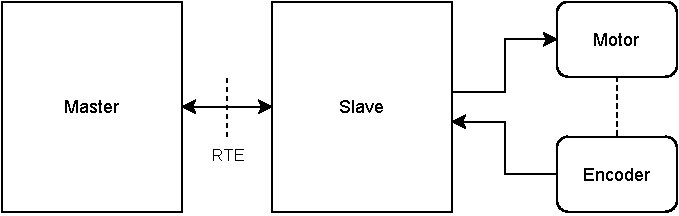
\includegraphics[width=0.8\linewidth]{overall-architecture.pdf}
	\end{figure}
\end{frame}
	\begin{frame}{Arquitetura do Sistema - Dispositivo \emph{Slave}}
	\begin{figure}
		\centering
		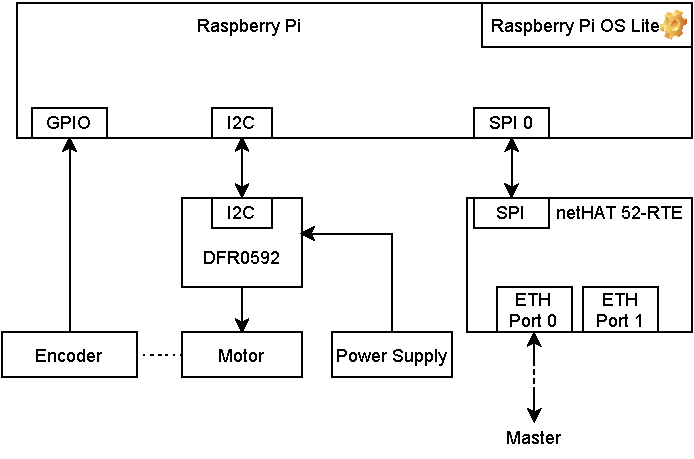
\includegraphics[width=0.8\linewidth]{slave_architecture.pdf}
	\end{figure}
\end{frame}
	\begin{frame}{Arquitetura do Sistema - Dispositivo \emph{Slave}}
	\begin{figure}
		\centering
		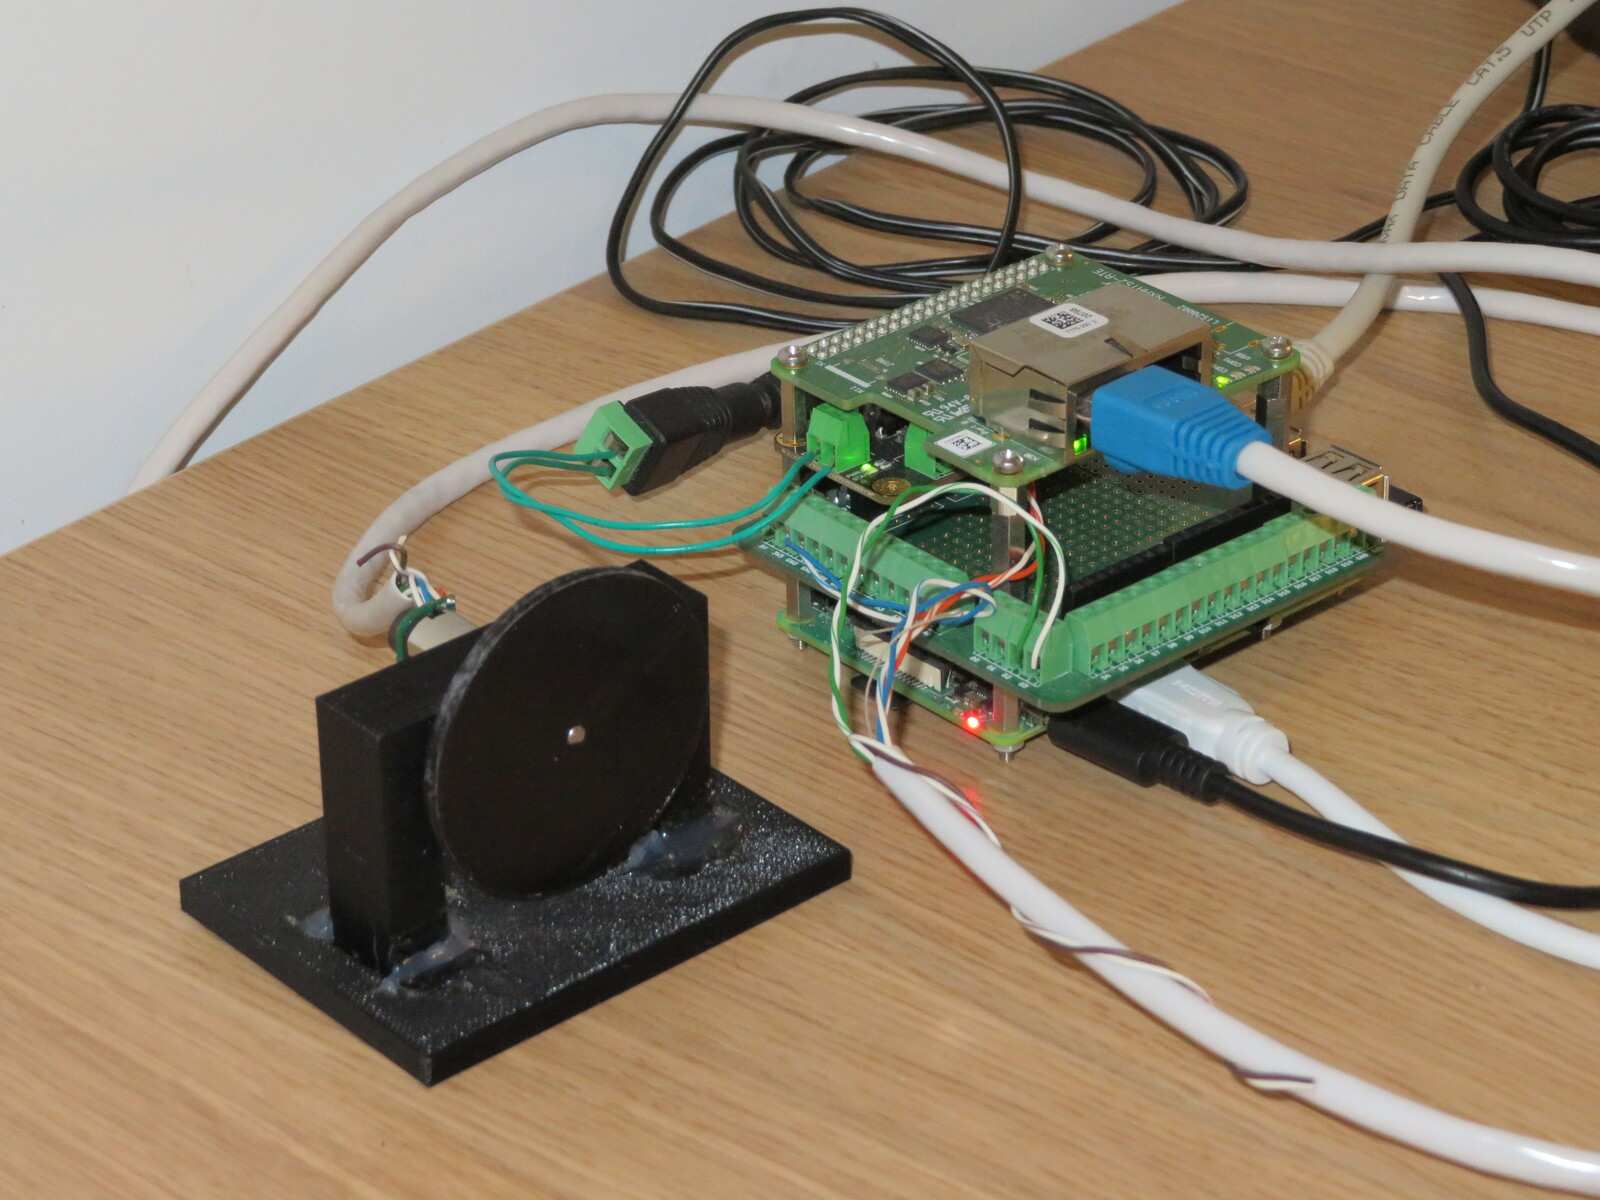
\includegraphics[width=0.75\linewidth]{hardware_overview.JPG}
	\end{figure}
\end{frame}
	\begin{frame}{Arquitetura do Software}
	\begin{figure}
		\centering
		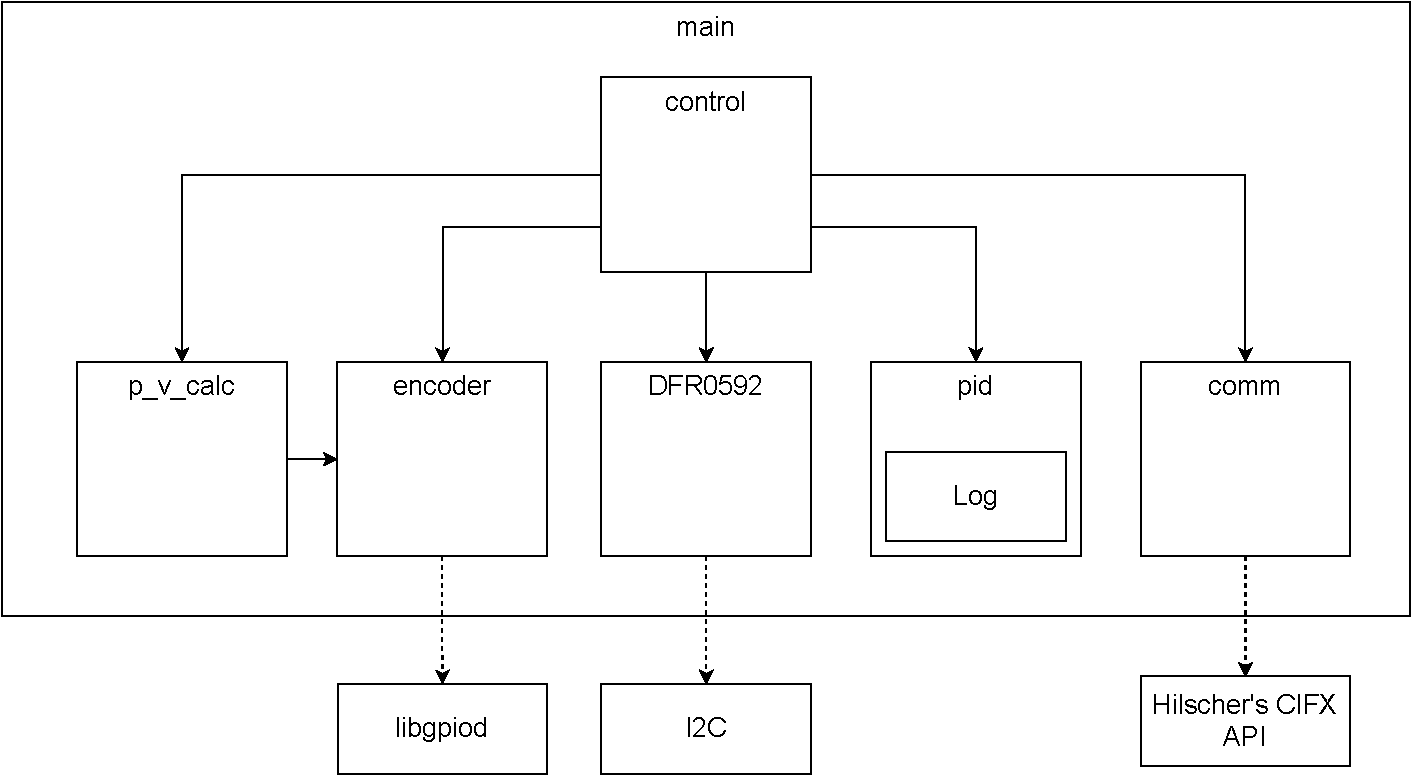
\includegraphics[width=\linewidth]{sw-architecture.pdf}
	\end{figure}
\end{frame}
	\begin{frame}{Controlo Local}
	\begin{figure}
		\centering
		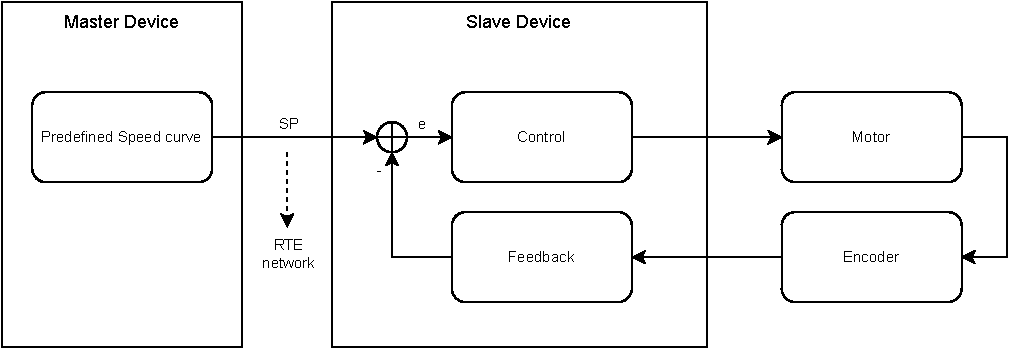
\includegraphics[width=\linewidth]{local-control.pdf}
	\end{figure}
\end{frame}
	\begin{frame}{Controlo Remoto}
	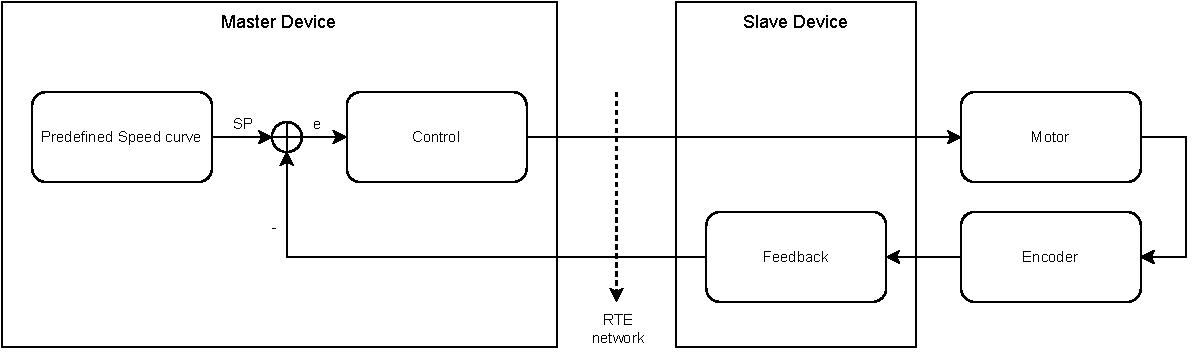
\includegraphics[width=\linewidth]{remote-control.pdf}
\end{frame}
	
	\begin{frame}{Resultados experimentais - comportamento do sistema}
	\centering
	\large
	Controlo remoto com per\'{i}odo de controlo de 10ms
	\begin{columns}
		\begin{column}{0.5\textwidth}
			\begin{figure}
				\centering
				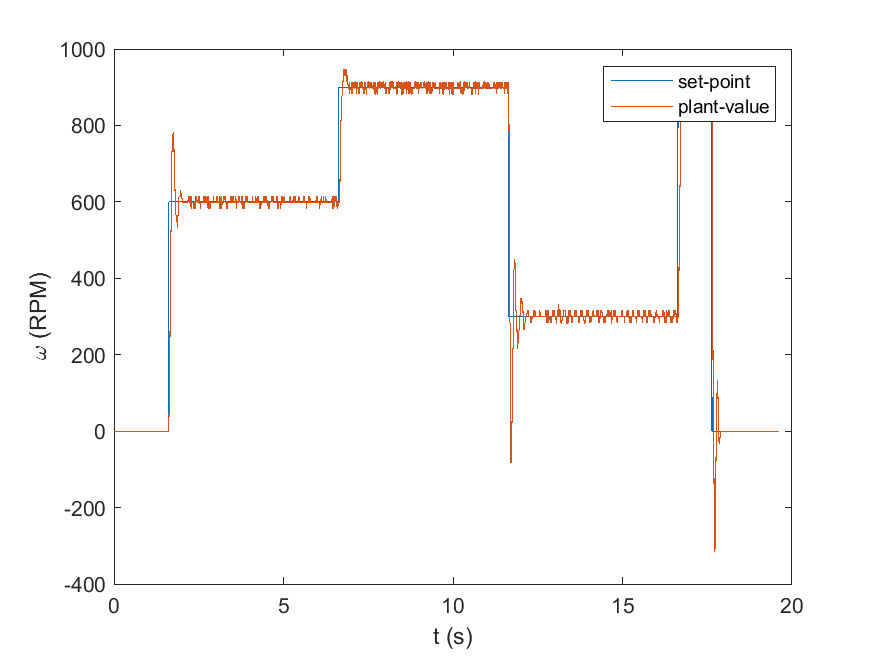
\includegraphics[width=\textwidth]{remote-5ms.png}
			\end{figure}
			\centering\normalsize
			Comportamento do sistema com per\'{i}odo de rede de 5ms
		\end{column}
		\begin{column}{0.5\textwidth}
			\begin{figure}
				\centering
				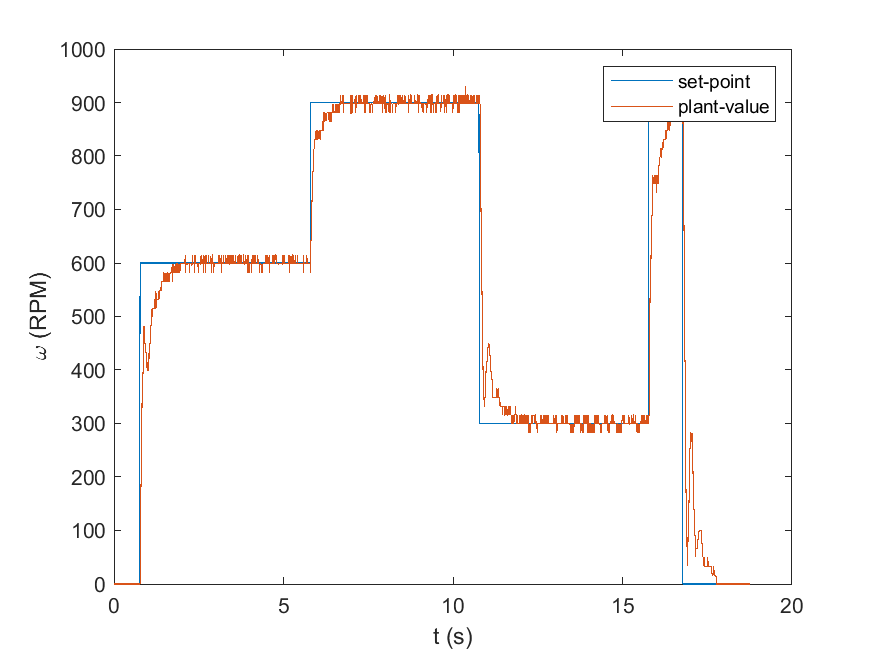
\includegraphics[width=\textwidth]{remote-20ms.png}
			\end{figure}
			\centering\normalsize
			Comportamento do sistema com per\'{i}odo de rede de 20ms
		\end{column}
	\end{columns}
\end{frame}
	\begin{frame}{Resultados experimentais - An\'{a}lise de Dados}
	\centering
	An\'{a}lise da resposta do sistema ao degrau
	\begin{table}
		\centering
		\resizebox{\linewidth}{!}{
			\begin{tabular}{|c|c|c|c|c|c|}
				\hline
				Test Case   & rise-time (s) & settling-time (s) & overshoot (\%) & peak (RPM) & peak time (s) \\
				\hline
				local-5ms   & 0.0366 & 1.8327 & 11.1124 & 664.9058 & 1.7327 \\
				\hline
				remote-5ms  & 0.0597 & 1.9769 & 30.555 & 781.2768 & 1.7626 \\
				\hline
				local-10ms  & 0.0544 & 5.1091 & 0.0301 & 615.2382 & 4.4606 \\
				\hline
				remote-10ms & 0.0434 & 5.1745 & 24.3232 & 764.6893 & 1.4324 \\
				\hline
				local-20ms  & 0.0472 & 4.7729 & 5.5528 & 631.6609 & 4.7700 \\
				\hline
				remote-20ms & 0.6024 & 5.1745 & 0.0902 & 615.5647 & 4.1693 \\
				\hline
			\end{tabular}
		}
	\end{table}
\end{frame}
	
	\begin{frame}{Conclus\~{o}es}
	\begin{itemize}
		\item Simplicidade $\Rightarrow$ M\'{i}nima influ\^{e}ncia externa;
		\item Os objetivos propostos foram atingidos;
		\item O sistema desenvolvido demonstra ser uma base s\'{o}lida para o desenvolvimento de m\'{o}dulos que explorem conceitos distintos;
	\end{itemize}
\end{frame}
	
\end{document}